\section{The Discovery of $CP$ violation \cite{Kaonen}}
The $CP$ asymmetry was discovered in the kaon sector at the Finch experiment in 1964. And was in important step towards the understanding of the weak interaction. The origin of the $CP$ violation was explained in the CKM matrix assuming that three or more quark generations exist.

\subsection{Theoretical principles}
In the years prior to the discovery of CP violation, parity and charge conjugation violations due to the weak interaction were observed, but there was no evidence of CP violation. At this time were just three quarks known the $u$, $d$ and $s$. Only in 1964 the $c$quark was postulated to explain the suppression of FCNC. The mass eigenstates $K^0$ and $\bar{K}^0$ have the same $CP$ eigenvalue. This lead to the conclution that the $CP$ eigenstates are a linear combination of both mass eigenstates:
\begin{align*}
    \left|K_1 \right> &= \frac{1}{\sqrt{2}} \left(\left|K^0\right> +
                        \left|\bar{K}^0\right> \right) \\
    \left|K_2 \right> &= \frac{1}{\sqrt{2}} \left(\left|K^0\right> -
                        \left|\bar{K}^0\right> \right)
\end{align*}
To conserve the $CP$ symmetry $K_1$ can only decay into two pions, while $K_2$ decays into three pions. Since the decay into three pions needs more phase space, the lifetime of the $K_2$ is longer as the one of the $K_1$. This is the reason for the identifictaion $K_L =K_2$ (L=long) and $K_S =K_1$ (S=short). The mesons $K^0$ and $\bar{K}^0$ also interact different with matter. While the $K^0$ mainly contributes to scattering processes, the $\bar{K}^0$ produces additional excitations of hyperons. This reason leads to a higher cross section and is the reason, that a part of the $K_L$ transitions to $K_S$. This was the idea for the measurment of the Finch experiment and would prove the $CP$ violation in weak interactions.

\subsection{The Cronin-Fitch Experiment}
The Cronin-Fitch experiment took place at the Brookhaven National Labratory. The idea was to place the detector far away from the interaction point, so all reminding Kaons are $K_L$. If then a decay into two pions would have been observed, that would be a  measurement of indirect $CP$ violation.\\
The experiment is assambled out of a two-armed spectrometer and a helium bag to reduce possible interactions. The spectrometer arms contain a spark-chamber before and behind a magnet and use a scintillator together with a water Cherenkov counter as a trigger. The principle of the measurement was to measure the angle $\vartheta$, where the sum of the momenta comes together. The second idea is to check that deposited energy is around the kaon mass. They observed a peak at $\cos(\vartheta) = 1$ compared to the Monte Carlo data. This lead to the branching $BR(K^0_L\rightarrow \pi^+\pi^-) = (2.0\pm0.4)\cdot 10^{-3}$. This is a clear observation of a two-body decay of $K_L$ and proves $CP$ violation.
The actual $CP$ eigenstates are
\begin{align*}
  \left|K_S \right> &= \frac{1}{\sqrt{1 + |\epsilon|^2}}(\left|K_1 \right> - \epsilon \left|K_2 \right>) \\
  \left|K_L \right> &= \frac{1}{\sqrt{1 + |\epsilon|^2}}(\left|K_2 \right> + \epsilon \left|K_1 \right>) \, .
\end{align*}
that allow a indirect measurement of the $CP$ violation with $\epsilon =(2.228\pm0.011)\cdot10^{-3}$. A direct observation of $CP$ violation by proving that $\Gamma(K_0\rightarrow \pi\pi)\neq \Gamma(\bar{K}_0\rightarrow \pi\pi)$ was done by NA48 at CERN and KTeV at Fermilab in 1999. The third type of $CP$ violation oigins from the interference between mixing and decay. The corresponding eigenstates are $\ket{M_L}$ and $\ket{M_H}$ corresponding to states with a \textbf{l}ow and \textbf{h}igh mass. $\ket{M_{L/H}} = p \ket{M_0} \pm q \ket{\bar{M}_H}$ with $|p|^2+|q|^2 = 1 $.
This eigenstates play a significant role for $B$ mesons.

\subsection{CKM Matrix and the $B$ meson sector}
In 1963 Cabibbo postulated a matrix, which could describe the mixing ot two quarks. In 1973 Kobayashi and Maskawa extended the matrix with a third quark generation. This lead to three mixing angles and a complex phase that could explain the $CP$ violation. In the Standard Model quarks get their masses trough Yukawa interaction. The non-diagonal Yukawa matrices can be diagonalized with unitary matrices. This leads to a change into the flavour base. The problem is that the Yukawa matrices for up- and down-type quarks cannot be diagonalized together. The remaining component is the CKM matrix, which is a unitar matrix as well.\\
The experimental results for the mixing angles are $\vartheta_{13} \ll \vartheta_{23} \ll \vartheta_{12} \ll 1$. Since the complex phase only occurs with $\sin\vartheta_{13}$, the $CP$ violation is highly suppressed. Because of the unitar nature of CKM matrix, there are different unitarity triangles that can be constructed from this condition. These can be measured precisely with $B$ mesons, since they have lower hadronic uncertainties and a higher sensitivity for the unitary angles. The CKM matrix predicted a large asymmetry in $B\bar{B}$ oscillations. They were dominated from $m_t^2|V_{tb}V_{td}|^2$ contributions. In the 1990s they build the first \textit{B factories} at $e^+e^-$ collidern. In 2001 BABAR and BELLE confirmed the $CP$ violation in the $B$ sector.\\
$CP$ violation was measured over the time difference between the $B^0$ and the $\bar{B}^0$ decay. The $B^0\bar{B}^0$ pair is produced highly boosted. One decay channel gets fully reconstructed and one is favour tagged, since the pair builds an entangled quantum state. The violation can be measured with the number of $B^0$ and $\bar{B}^0$ mesons decaying into a final, $CP$ eigenstate f.
\begin{align*}
	A_{CP}(f,t) = \frac{N(\bar{B}^0 \rightarrow f) - N(B^0 \rightarrow f)} {N(\bar{B}^0 \rightarrow f) + N(B^0 \rightarrow f)} = S_F \sin(\Delta m t) -C_F \cos(\Delta m t)
\end{align*}
The prefactors $S_F$ and $C_F$ depend on the decay mode and can be used to determine the unitarity triangle.
\begin{figure}
	\center
  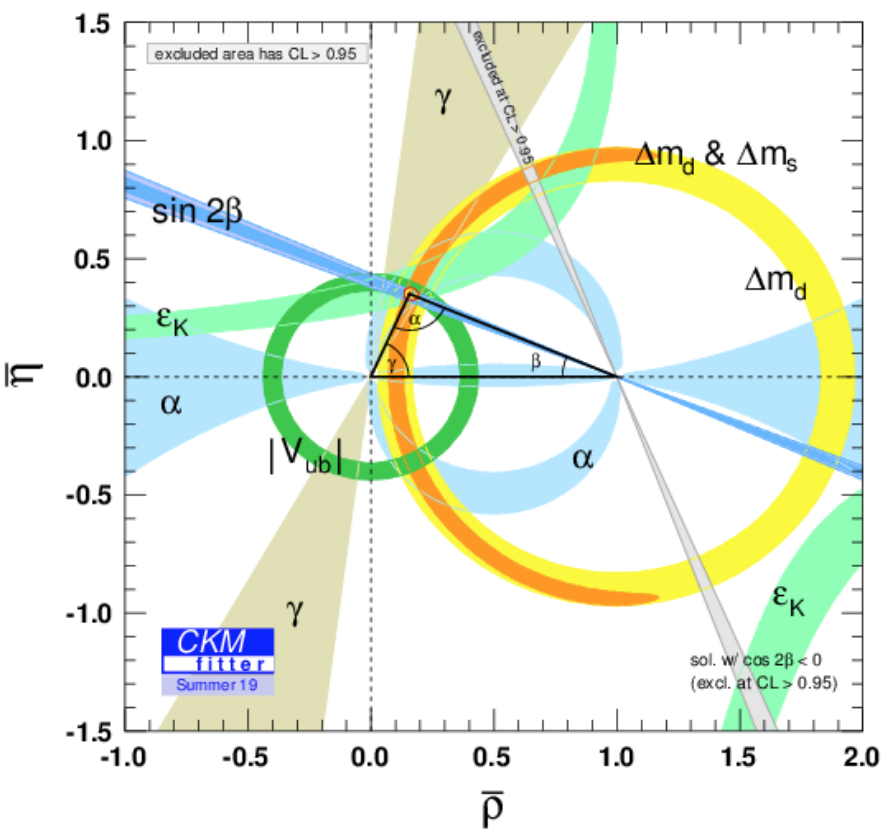
\includegraphics[width=0.35\textwidth]{graphics/CKM.png}
  \caption{Global average for one unitary triangle. \cite{Kaonen}}
	\label{fig:CKM}
\end{figure}
The combined results of all current measurements is shown in figure \ref{fig:CKM}. Currently all measurements are in agreement. \\
The Jarlskog invariant measures the strength of the $CP$ violation:
\begin{align}
	J = 2 A_{\Delta} = (3.060^{+0.071}_{-0.079}) \cdot 10^{-5}
\end{align}
Besides the observation of $CP$ violation in $B^0\bar{B}^0$ systems, it was also possible to determine it in $B_s$ and $D$ systems.\\
Furture experiments aim for higher precisions in determining the different parameter of the unitarity trianle. Beside this there will be also studies for $CP$ violation in the leptonic sector. Due to the small size of SM $CP$ violation it is also not able to answer the question of the matter-antimatter asymmetry of our universe.
